% =========================================================
\section{Sistema de automatización desarrollado}
\label{sec:sistema}
% =========================================================

El software se desarrolló como una aplicación de escritorio en
Python~3.12 con interfaz gráfica basada en \texttt{PySide6}~6.11, el
enlace oficial de Qt~6 para Python. La arquitectura sigue un patrón
modular en el que cada subsistema de hardware corresponde a un paquete
independiente, y la interfaz gráfica actúa como coordinador de alto
nivel.

\subsection{Arquitectura modular}
\label{sec:arquitectura}

El proyecto se organiza en torno a un paquete principal \texttt{app/}
que agrupa los siguientes módulos:

{\sloppy
\begin{itemize}
  \item \texttt{app/laser/control\_laser.py} — gestión de la conexión
    con el láser mediante la biblioteca de enlace dinámico
    \texttt{REMOTECONTROL64.dll}. Expone una interfaz pública de
    operación (\texttt{start}, \texttt{stop}, \texttt{leer\_estado},
    \texttt{ping}, \texttt{modo\_seguro}), de lectura
    (\texttt{read\_output\_level}, \texttt{read\_eo\_delay},
    \texttt{read\_burst\_mode}, \texttt{read\_cooling\_temp},
    \texttt{read\_pulse\_counter}, \texttt{leer\_parametros}) y de
    escritura (\texttt{set\_output\_level}, \texttt{set\_eo\_delay},
    \texttt{set\_burst\_mode}, \texttt{set\_burst\_length},
    \texttt{set\_cooling\_temp}); el acceso directo a registros queda
    encapsulado y no se invoca desde la interfaz gráfica.

  \item \texttt{app/osciloscopio/control\_osciloscopio.py} —
    comunicación VXI-11 con el osciloscopio; implementa la consulta de
    parámetros de adquisición, la configuración del modo de acumulación
    de cada secuencia, la transferencia binaria de forma de onda, la
    lectura del preámbulo necesario para la conversión a unidades
    físicas y la verificación de que cada registro leído corresponde a
    una adquisición nueva (\cref{sec:verificacion_adquisicion}).

  \item \texttt{app/temperatura/temperatura.py} — hilo de lectura
    continua de los cuatro sensores DS18B20 conectados al módulo
    ESP32~WROOM-32; mantiene la última lectura en memoria, indica si el
    valor es reciente y emite señales Qt cuando se actualiza. El
    firmware del módulo se conserva en \texttt{esp32/temperatura/}.

  \item \texttt{app/medicion/medicion.py} — fachada de hardware y
    orquestador de la secuencia de medición automática; coordina el
    láser, el osciloscopio y el módulo de temperatura según el modo de
    operación seleccionado, y emite advertencias sin interrumpir la
    secuencia.

  \item \texttt{app/medicion/trigger.py} — lógica de disparo; evalúa
    la condición de inicio y fin de adquisición en función de la
    temperatura o del tiempo según el modo activo.

  \item \texttt{app/almacenamiento/almacenamiento.py} — persistencia
    de datos; guarda las muestras crudas en archivos \texttt{.npy}, los
    metadatos de cada medición en un registro \texttt{.csv} de sesión y
    las condiciones generales en \texttt{metadatos\_sesion.txt}.

  \item \texttt{app/conexion/monitoreo.py} — hilo de monitoreo de
    conexión; comprueba periódicamente el estado de cada dispositivo,
    intenta la reconexión y actualiza los indicadores de la interfaz.
    El módulo vecino \texttt{prueba\_conexion.py} sondea los
    dispositivos con valores de conexión que todavía no se han
    guardado.

  \item \texttt{app/modo\_seguro/modo\_seguro.py} — procedimiento de
    seguridad descrito en la \cref{sec:auto_laser}; desactiva el láser
    de forma controlada ante una parada de emergencia, un fallo de
    comunicación o la conclusión de la secuencia.

  \item \texttt{app/exportacion/exportar\_mat.py} — conversión de una
    sesión completa al formato \texttt{.mat} para su análisis
    posterior en MATLAB.

  \item \texttt{app/gui/} — conjunto de ventanas y componentes
    gráficos: la bienvenida (\texttt{bienvenida.py}), las tres
    ventanas de operación, la pestaña de visualización
    (\texttt{visualizacion.py}) y el diálogo de conexión
    (\texttt{dialogo\_conexion.py}).

  \item \texttt{app/config.py}, \texttt{app/config\_local.py} y
    \texttt{app/config\_usuario.py} — parámetros de conexión (puertos
    serie del ESP32 y del láser, dirección IP del osciloscopio). Se
    leen con el orden de prioridad: archivo JSON del usuario, guardado
    fuera del repositorio desde el diálogo de conexión; después
    \texttt{config\_local.py}, propio de cada computadora y no
    versionado; y por último los valores por omisión de
    \texttt{config.py}. Si el JSON no existe o está dañado, la
    aplicación arranca con los valores siguientes en ese orden.
\end{itemize}
\par}

El punto de entrada de la aplicación es \texttt{main.py}, ubicado en la
raíz del proyecto, que aplica la configuración de conexión, instancia
la ventana de bienvenida y entrega el control al ciclo de eventos de
Qt. En la computadora del laboratorio se ejecuta mediante
\texttt{iniciar.bat}, que lanza \texttt{main.py} con el intérprete del
entorno virtual del proyecto y mantiene abierta la consola si la
aplicación termina con error, de modo que el operador no necesita
abrir una terminal. Fuera de \texttt{app/}, la carpeta
\texttt{herramientas/} reúne los programas auxiliares de verificación
y prueba (\texttt{verificar\_sesion.py}, \texttt{simular\_barrido.py},
\texttt{generar\_sesion\_prueba.py}, \texttt{prueba\_buffer.py}, entre
otros) y \texttt{codigos\_de\_prueba/} las pruebas de la interfaz sin
hardware; ambos se describen en la \cref{sec:validacion}.

La \cref{fig:arquitectura} resume esta organización y las relaciones
entre los módulos. El de medición ocupa la posición central: coordina la
secuencia, consulta a los tres instrumentos y escribe en el registro de
sesión las mediciones automáticas; la captura manual guarda sus filas
desde la interfaz, con el mismo módulo de almacenamiento. El de
conexión y monitoreo no participa en la secuencia; vigila el estado de
los enlaces de forma continua y en paralelo, de modo que la pérdida de
un dispositivo se detecta también fuera de una medición en curso.

El monitoreo no trata igual a los tres dispositivos. Del láser lee
activamente el registro \texttt{State}; del osciloscopio consulta la
bandera de conexión que mantiene su controlador, sin enviar una orden
al instrumento; del ESP32 comprueba que la última lectura recibida sea
reciente. El ciclo se repite cada \SI{5}{\second} en reposo y cada
\SI{1}{\second} durante una secuencia, y se suspende mientras dura una
captura para no competir con la transferencia de la forma de onda.
Cuando un dispositivo no responde, su indicador pasa a amarillo y se
lanzan hasta tres intentos de reconexión en un hilo propio; si fallan,
el indicador pasa a rojo. Solo la pérdida del láser o del osciloscopio
activa el modo seguro: el ESP32 no es crítico para la seguridad del
haz, y su ausencia se registra en cada medición afectada
(\cref{sec:secuencia}).

% =========================================================
% Figura: arquitectura de módulos del sistema de automatización
% Requiere en el preámbulo:
%   \usepackage{tikz}
%   \usetikzlibrary{positioning,arrows.meta,fit,backgrounds}
% =========================================================

\begin{figure}[htbp]
  \centering
  \begin{tikzpicture}[
      font=\footnotesize,
      modulo/.style={
        draw, rounded corners=2pt, align=center,
        text width=30mm, minimum height=11mm, inner sep=2pt},
      hw/.style={modulo, fill=black!6},
      capa/.style={
        draw=black!35, dashed, rounded corners=4pt, inner sep=4mm, inner ysep=5mm},
      etiqueta/.style={font=\scriptsize\itshape, text=black!55},
      flecha/.style={-{Stealth[length=2mm]}, thick},
      pasiva/.style={-{Stealth[length=2mm]}, densely dashed, black!55},
      node distance=8mm and 10mm
    ]

    % --- Presentación ---
    \node[modulo] (gui) {Interfaz gráfica\\\scriptsize eventos y presentación};

    % --- Coordinación ---
    \node[modulo, below=14mm of gui] (med)
      {Medición\\\scriptsize orquestación de la secuencia};
    \node[modulo, left=of med] (conn)
      {Conexión y monitoreo\\\scriptsize estado y reintentos};
    \node[modulo, right=of med] (trig)
      {Disparo\\\scriptsize por tiempo o temperatura};

    % --- Hardware ---
    \node[hw, below=14mm of med] (oscil)
      {Osciloscopio\\\scriptsize VXI-11 sobre Ethernet};
    \node[hw, left=of oscil] (laser)
      {Láser\\\scriptsize RS-232};
    \node[hw, right=of oscil] (temp)
      {Temperatura\\\scriptsize ESP32 y sensores};

    % --- Datos y seguridad ---
    \node[modulo, below=14mm of oscil] (store)
      {Almacenamiento\\\scriptsize registro de sesión};
    \node[modulo, left=of store] (safe)
      {Modo seguro\\\scriptsize solo actúa sobre el láser};
    \node[modulo, right=of store] (viz)
      {Visualización\\\scriptsize consulta y exportación};

    % --- Cajas de capa ---
    \begin{scope}[on background layer]
      \node[capa, fit=(conn)(med)(trig)] (cap_coord) {};
      \node[capa, fit=(laser)(oscil)(temp)] (cap_hw) {};
      \node[capa, fit=(safe)(store)(viz)] (cap_datos) {};
    \end{scope}

    \node[etiqueta, anchor=north west] at ([xshift=1mm,yshift=-0.5mm]cap_coord.north west) {coordinación};
    \node[etiqueta, anchor=north west] at ([xshift=1mm,yshift=-0.5mm]cap_hw.north west) {instrumentos};
    \node[etiqueta, anchor=north west] at ([xshift=1mm,yshift=-0.5mm]cap_datos.north west) {datos};

    % --- Flujo de control ---
    \draw[flecha] (gui) -- node[right, font=\scriptsize] {modo automático} (med);
    \draw[flecha] (gui.west) -- ++(-2.2,0) |- (conn.north);
    \draw[flecha] (med) -- (trig);
    \draw[flecha] (med) -- (oscil);
    \draw[flecha] (med.south west) -- (laser.north east);
    \draw[flecha] (med.south east) -- (temp.north west);
    \draw[flecha] (trig.south) -- (temp.north);
    \draw[flecha] (oscil) -- (store);
    \draw[flecha] (med.north west) -- ++(-0.35,0) -- ++(0,-0.4)
      -| ([xshift=-6mm]cap_hw.west) |- (safe.west);

    % --- Vigilancia pasiva ---
    \draw[pasiva] (conn.south) -- (laser.north);
    \draw[pasiva] (conn.south east) -- (oscil.north west);
    \draw[pasiva] (conn.east) -- ++(0.3,0) -- ++(0,-0.55)
      -| ([xshift=6mm]temp.north east) -- ([xshift=6mm]temp.north east|-temp.east) -- (temp.east);

    % --- Modo seguro ---
    \draw[flecha] (safe) -- (laser);

    % --- Consulta ---
    \draw[flecha] (store) -- (viz);

  \end{tikzpicture}
  \caption[Arquitectura de módulos del sistema de automatización]{%
    Arquitectura de módulos del sistema de automatización. Las flechas
    continuas indican control o transferencia de datos; las discontinuas,
    la vigilancia pasiva del estado de conexión. El módulo de medición
    coordina la secuencia y es el único que escribe en el registro de
    sesión. El modo seguro actúa exclusivamente sobre el láser: la
    configuración del osciloscopio no se modifica desde el programa.}
  \label{fig:arquitectura}
\end{figure}


\subsection{Decisiones de diseño}
\label{sec:decisiones}

La elección de \texttt{PySide6} frente a otras bibliotecas gráficas
responde a tres criterios: compatibilidad nativa con Qt~6, soporte
activo de largo plazo por parte de The Qt Company, y disponibilidad del
módulo \texttt{pyqtgraph} para visualización en tiempo real sin pérdida
de rendimiento.

Todas las operaciones de hardware se ejecutan en hilos secundarios
(\texttt{QThread}) independientes del hilo principal de la interfaz.
Esta separación es obligatoria en aplicaciones Qt: bloquear el hilo
principal durante una transferencia de forma de onda o una espera de
conexión provoca que la ventana quede sin respuesta. Cada hilo comunica
su resultado al hilo principal mediante señales Qt (\texttt{Signal}),
que Qt entrega de forma segura entre hilos.

El control del láser mediante \texttt{ctypes} directo, en lugar de un
subproceso separado o una capa intermedia, obedece a la restricción de
arquitectura de la \texttt{DLL}: la biblioteca
\texttt{REMOTECONTROL64.dll} es exclusivamente de 64~bits y debe
cargarse en el mismo espacio de proceso que el intérprete de Python. El
uso de \texttt{ctypes.WinDLL} desde Python~3.12 de 64~bits satisface
esta condición sin dependencias adicionales.

La configuración de los ejes y del disparo del osciloscopio se opera en
modo de solo lectura desde la aplicación. Las escalas vertical y
horizontal, el acoplamiento, el nivel de disparo y la longitud de
registro se configuran físicamente en el instrumento y el programa
únicamente los consulta y los registra junto con cada medición. Esta
decisión responde a un criterio de trazabilidad: si el programa pudiera
modificar esa configuración, los metadatos guardados describirían lo
que el programa creyó haber establecido y no necesariamente lo que el
instrumento aplicó. Al consultar en lugar de escribir, el osciloscopio
es la única fuente de verdad sobre la calibración de sus propios ejes.
La aplicación sí escribe los parámetros que gobiernan la acumulación y
la transferencia, que no alteran esa calibración: el modo de
adquisición (\texttt{ACQ:MODE}), el número de promedios
(\texttt{ACQ:NUMAVG}), la condición de detención
(\texttt{ACQ:STOPAFTER}), el inicio y la detención de la adquisición
(\texttt{ACQ:STATE}) y el canal de origen de los datos
(\texttt{DATA:SOURCE}). Al cerrar una secuencia automática, el
instrumento recupera el modo de adquisición y el número de promedios
que tenía antes de iniciarla. En la \cref{sec:trabajo_futuro} se
discute la reincorporación del control de escalas como mejora
propuesta.

Los alcances de la validación con el osciloscopio y los canales
empleados se describen en la \cref{sec:equipos}. La respuesta completa a la consulta
\texttt{*IDN?}, junto con el modelo y el canal en uso, se guarda en el
archivo \texttt{metadatos\_sesion.txt} de cada sesión
(\cref{sec:formato_datos}), de modo que el instrumento empleado queda
documentado en los propios datos.

Una anomalía que afecta a una sola medición no detiene la secuencia.
Una lectura de temperatura ausente, un sensor que deja de responder o
una captura sin adquisición nueva se registran en la fila
correspondiente mediante \texttt{error\_flag} y \texttt{error\_desc},
y se notifican al operador como advertencia; la secuencia continúa con
el siguiente punto. Interrumpirla en esos casos desecharía las
mediciones válidas que aún pueden obtenerse de una muestra cuyo
enfriamiento no se puede repetir a voluntad, mientras que la marca en
el registro permite excluir después la medición afectada. La secuencia
se aborta solo cuando no puede continuar con sentido: si el láser no
arranca, si el osciloscopio rechaza la configuración del modo, o si en
modo temperatura la lectura falta durante más de \SI{300}{\second}
(\cref{sec:secuencia}).

La última decisión de esta subsección no es de software, pero condiciona
lo que el software puede informar. Los cuatro sensores de temperatura
admiten compartir un mismo bus 1-Wire, que es su modo de empleo
habitual; en este montaje cada uno ocupa un bus propio, según se muestra
en la \cref{fig:modulo_temperatura}. La razón es de diagnóstico: sobre
un bus compartido, la caída de un sensor se manifiesta como una lectura
ausente entre varias y exige identificar cuál falló; con buses
separados, la línea que deja de responder nombra al dispositivo sin
ambigüedad. Esa correspondencia es la que permite que el registro de
sesión consigne qué sensor se perdió y no solo que se perdió alguno,
como se documenta en la \cref{sec:falla_temperatura}.

\subsection{Interfaz gráfica}
\label{sec:gui}

La interfaz ofrece tres modos de operación seleccionables desde una
ventana de bienvenida: control exclusivo del láser, control exclusivo
del osciloscopio, y modo combinado que habilita la secuencia de
medición automática. Cada modo abre una ventana independiente; al
cerrarla, la aplicación regresa a la bienvenida sin necesidad de
reiniciar el proceso.

La bienvenida incluye además el botón \textit{Conexión}, que abre un
diálogo para elegir el puerto serie del ESP32, el del láser y la
dirección IP del osciloscopio sin editar el código. El botón
\textit{Probar conexión} sondea los dispositivos con los valores
escritos en el diálogo, en un hilo aparte y sin guardarlos; al aceptar,
los valores se escriben en el archivo JSON del usuario y quedan
vigentes para la siguiente conexión y para los arranques posteriores.
El mismo diálogo está disponible en la barra superior de la ventana
principal, donde se deshabilita mientras el láser está en
\texttt{RUN} o su estado no se ha podido confirmar, durante una
secuencia y durante una captura, para que un cambio de puerto no deje
sin control a un dispositivo activo.

Las ventanas de control individual, mostradas en la
\cref{fig:ventanas_individuales}, sirven para la puesta a punto previa
a una secuencia: alineación del arreglo, ajuste del nivel de salida del
láser y verificación de que el osciloscopio dispara y transfiere. Ambas
comparten con la ventana principal la barra de estado de conexión y el
botón de parada de emergencia. Las capturas de pantalla de esta
subsección corresponden a la interfaz de principios de septiembre de
2026; los elementos incorporados después se describen en el texto.

\begin{figure}[H]
  \centering
  \begin{subfigure}[t]{0.48\textwidth}
    \centering
    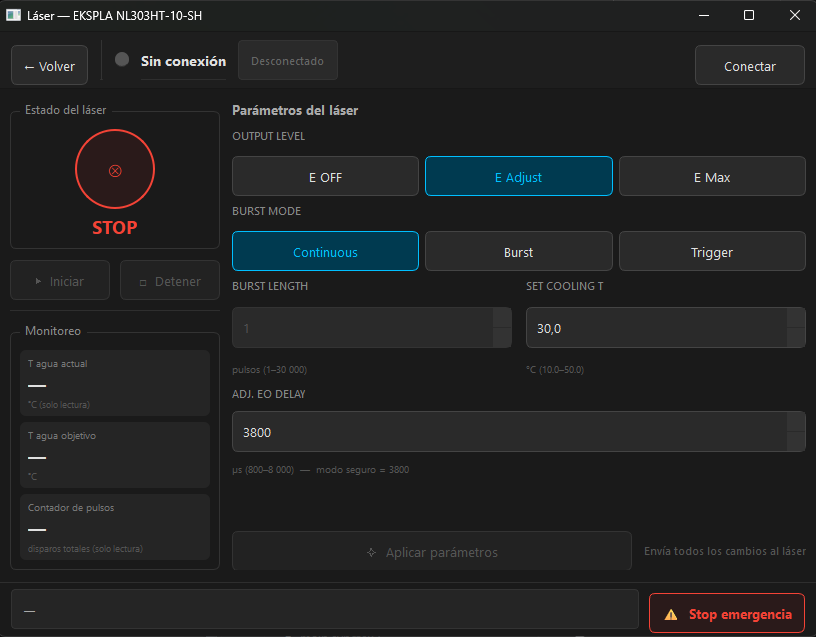
\includegraphics[width=\textwidth]{ventana_laser}
    \caption{Control del láser.}
    \label{fig:ventana_laser}
  \end{subfigure}
  \hfill
  \begin{subfigure}[t]{0.48\textwidth}
    \centering
    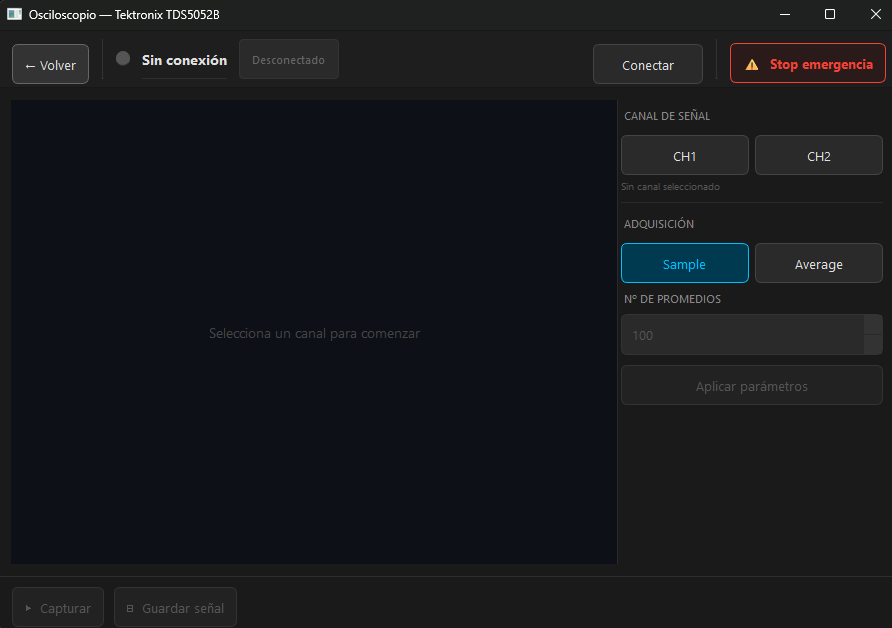
\includegraphics[width=\textwidth]{ventana_osciloscopio}
    \caption{Control del osciloscopio.}
    \label{fig:ventana_osciloscopio}
  \end{subfigure}
  \caption{Ventanas de control individual. La de la derecha muestra el
           bloque de escalas y disparo consultado al instrumento, que la
           aplicación no escribe; el modo de adquisición y el número de
           promedios sí se aplican desde esa ventana.}
  \label{fig:ventanas_individuales}
\end{figure}

La ventana principal del modo combinado
(\texttt{app/gui/ventana\_ambos.py}) se organiza en tres pestañas, que
se muestran en la \cref{fig:ventana_ambos}:

\begin{itemize}
  \item \textbf{Parámetros} (\cref{fig:ventana_ambos_parametros}) —
    configura los parámetros del láser (nivel de energía, modo de
    disparo, longitud de ráfaga, \textit{EO delay} y temperatura de
    consigna del enfriamiento, \textit{Set cooling}) y los aplica con
    un botón propio. El panel del osciloscopio permite elegir el canal
    de la señal (CH1 o CH2) y el modo de adquisición
    (\textit{Sample} o \textit{Average}, con su número de promedios),
    que se envían con \textit{Aplicar parámetros}, y muestra en modo
    de solo lectura las escalas y el disparo vigentes. Debajo, el panel
    \textit{Geometría de la sesión} recoge la separación entre el
    hidrófono y el haz y el volumen vertido.

  \item \textbf{Medición} (\cref{fig:ventana_ambos_medicion}) — reúne
    la captura manual (\textit{Capturar} y \textit{Guardar}) y los
    controles de la secuencia automática: el modo (por tiempo o por
    temperatura), sus parámetros (intervalo y número de mediciones, o
    temperatura inicial, final y paso), y los botones de inicio y de
    detención. La sesión se crea al guardar la primera captura manual,
    con la carpeta que elige el operador, o se reabre desde un registro
    existente; la secuencia automática solo se habilita con una sesión
    activa.

  \item \textbf{Visualizar datos} (\cref{fig:ventana_ambos_visualizacion})
    — presenta la lista de mediciones de la sesión y la forma de onda
    seleccionada en un gráfico interactivo de \texttt{pyqtgraph} con
    ejes calibrados en tiempo (\si{\micro\second}) y voltaje
    (\si{\milli\volt}). Sus botones permiten reabrir una sesión
    anterior (\textit{Abrir CSV\ldots}), copiar la carpeta de la
    sesión a otro destino (\textit{Exportar sesión\ldots}) y
    convertirla a formato \texttt{.mat} (\textit{Convertir a MATLAB}).
\end{itemize}

\begin{figure}[H]
  \centering
  \begin{subfigure}[t]{0.9\textwidth}
    \centering
    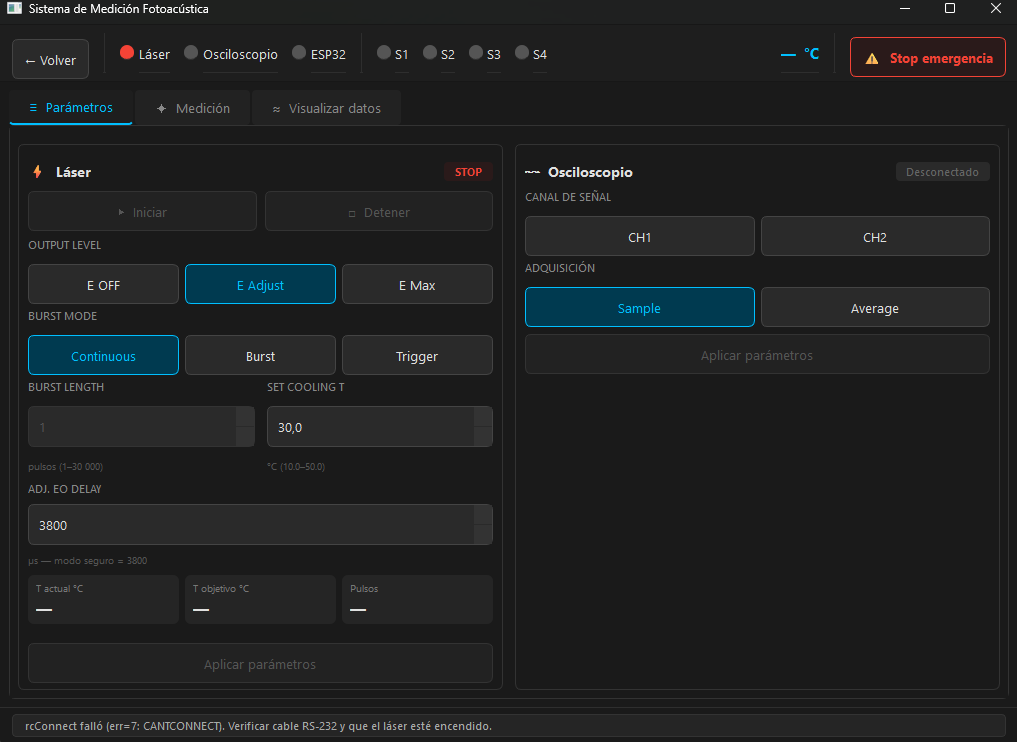
\includegraphics[width=\textwidth]{ventana_auto_1}
    \caption{Pestaña \textit{Parámetros}.}
    \label{fig:ventana_ambos_parametros}
  \end{subfigure}

  \vspace{0.6em}

  \begin{subfigure}[t]{0.9\textwidth}
    \centering
    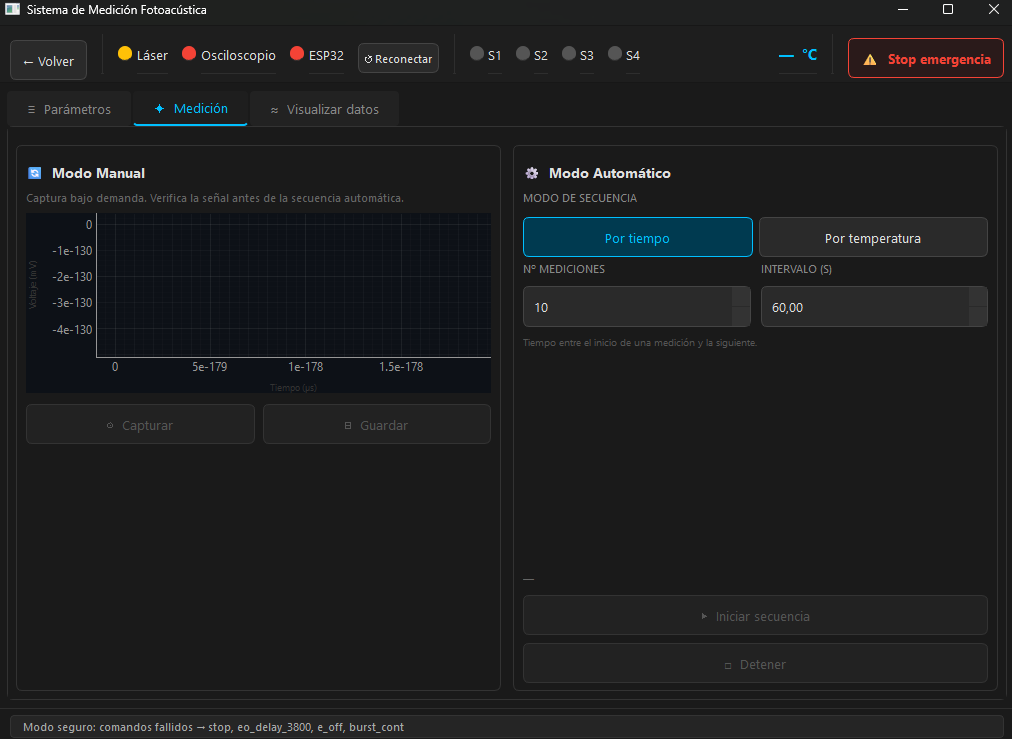
\includegraphics[width=\textwidth]{ventana_auto_2}
    \caption{Pestaña \textit{Medición}.}
    \label{fig:ventana_ambos_medicion}
  \end{subfigure}

  \vspace{0.6em}

  \begin{subfigure}[t]{0.9\textwidth}
    \centering
    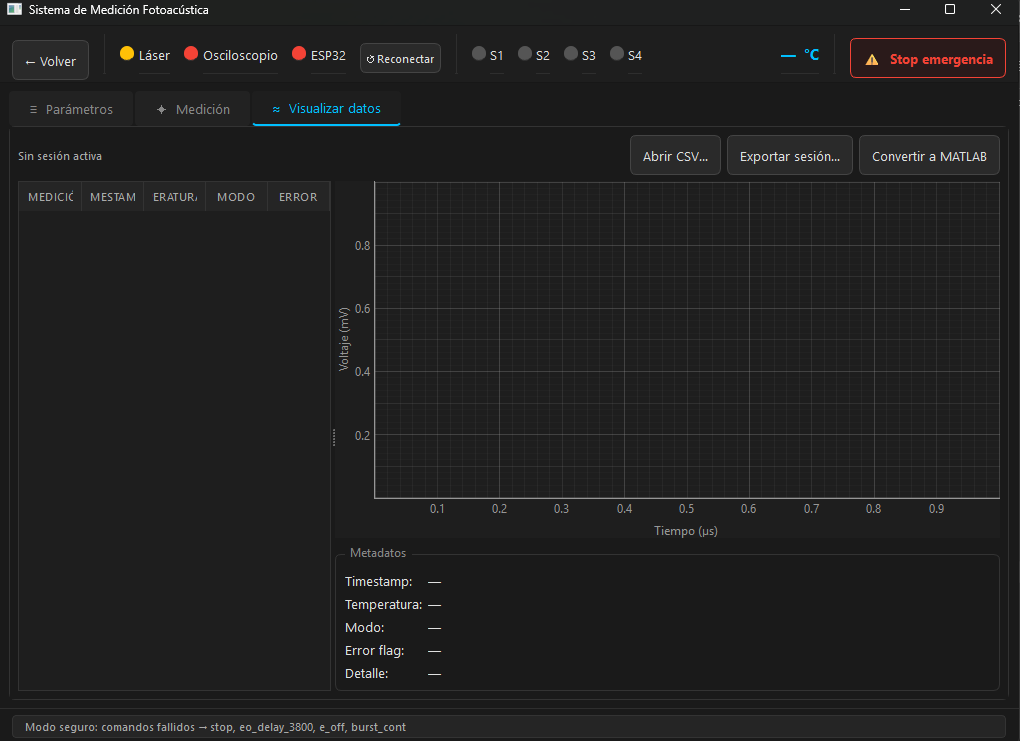
\includegraphics[width=\textwidth]{ventana_auto_3}
    \caption{Pestaña \textit{Visualizar datos}.}
    \label{fig:ventana_ambos_visualizacion}
  \end{subfigure}
  \caption{Ventana principal del modo combinado. La barra superior
           conserva en las tres pestañas los indicadores de conexión de
           los tres dispositivos, las lecturas de los cuatro sensores de
           temperatura y el botón de parada de emergencia.}
  \label{fig:ventana_ambos}
\end{figure}

La barra superior muestra el estado de conexión de cada dispositivo
(láser, osciloscopio, ESP32) mediante indicadores de color: verde para
conexión activa, amarillo mientras se intenta la reconexión o cuando
una captura terminó con advertencia, y rojo para desconectado. Cuando
el ESP32 queda desconectado aparece junto a su indicador el botón
\textit{Reconectar}, que se oculta al restablecerse la conexión. La
temperatura y el estado de los cuatro sensores se actualizan cada
segundo; si no hay una lectura reciente del ESP32, la temperatura se
sustituye por un guion y los indicadores de los sensores pasan a gris,
de modo que el último valor recibido no se presente como si
correspondiera a la muestra. El estado del láser se lee del registro
\texttt{State} cada segundo, con independencia de quién lo haya
cambiado: un arranque o una detención ordenados desde el control del
propio láser se reflejan en la interfaz sin intervención del operador.

\subsection{Protecciones de la operación}
\label{sec:protecciones}

Además del modo seguro del láser (\cref{sec:auto_laser}), la interfaz
incorpora un conjunto de bloqueos y confirmaciones cuyo propósito es
que ninguna acción del operador produzca un registro que no
corresponda a lo ocurrido. Los modos de falla que motivaron varios de
ellos se documentan en la \cref{sec:fallas}; aquí se describe su
diseño.

\begin{itemize}
  \item \textbf{Bloqueo durante la secuencia.} Mientras una secuencia
    automática está en curso, el worker de medición es el único que
    configura y lee el osciloscopio. Por ello se deshabilitan la
    selección de canal, el modo de adquisición, el número de promedios
    y su botón de aplicación, así como \textit{Capturar} y
    \textit{Guardar}, que escribiría en la sesión al mismo tiempo que
    el worker. También se bloquean la reapertura de sesiones, el
    cambio de modo automático y el diálogo de conexión. Al terminar o
    abortarse la secuencia, los controles se restablecen;
    \textit{Guardar} vuelve solo si quedó una captura manual sin
    guardar.

  \item \textbf{Geometría fija por sesión.} La separación
    hidrófono--haz y el volumen vertido se escriben en los metadatos
    al crear la sesión y no se vuelven a leer. Si falta alguno de los
    dos al capturar antes de que exista la sesión, se advierte al
    operador y se le ofrece llenarlo; una vez creada la sesión, los
    campos quedan deshabilitados con un aviso visible, para que un
    cambio posterior no parezca registrado.

  \item \textbf{Confirmación de sesión reabierta.} Una sesión abierta
    con \textit{Abrir CSV\ldots} puede ser de otro día. Antes de la
    primera escritura en ella, sea un \textit{Guardar} manual o una
    secuencia, la interfaz muestra la fecha de creación de la sesión y
    pide confirmación. Una respuesta afirmativa vale para el resto de
    esa reapertura; una negativa cancela solo esa escritura. En la
    secuencia, la pregunta se formula después de que el operador
    acepta iniciarla, de modo que la confirmación solo queda registrada
    si la secuencia efectivamente arranca.

  \item \textbf{Parada de emergencia, red de seguridad y modo
    degradado.} El botón de parada envía las órdenes de modo seguro al
    láser de forma inmediata, sin depender de que la secuencia
    responda, y solicita la detención del worker y del trigger. La
    interfaz no se libera hasta que ambos confirman su fin. Si esa
    confirmación no llega en \SI{150}{\second}, plazo elegido por
    encima del peor caso de una captura, que es de \SI{90}{\second},
    la interfaz se libera de todos modos y entra en modo degradado: no
    hay forma segura de comprobar que el hilo anterior terminó, de
    manera que \textit{Iniciar secuencia} y el regreso a la bienvenida
    quedan bloqueados y se pide al operador reiniciar la aplicación.

  \item \textbf{Validaciones previas a la secuencia.} La secuencia solo
    se inicia con el láser conectado y en \texttt{RUN}, el osciloscopio
    conectado y, en modo temperatura, el ESP32 conectado y un paso de
    temperatura mayor que cero. En modo tiempo se rechaza un intervalo
    menor que la duración estimada de una captura
    (\cref{sec:secuencia}). Superadas estas comprobaciones, un diálogo
    resume la configuración y pide confirmación.

  \item \textbf{Arranque del módulo de temperatura sin reinicio.} El
    puerto serie del ESP32 se abre con las líneas DTR y RTS en bajo,
    para no activar el circuito de reinicio automático de la placa, y
    a continuación se le envía la orden \texttt{START}, ya que el
    firmware conserva detenida la transmisión si la sesión anterior
    terminó con \texttt{STOP}.

  \item \textbf{Aviso de inactividad.} Con el láser en \texttt{RUN} y
    fuera de una secuencia, un minuto sin actividad del operador en la
    ventana abre un diálogo que pregunta si se sigue usando el láser;
    la respuesta negativa ejecuta la parada de emergencia. El diálogo
    espera la respuesta sin tiempo límite, de modo que, si nadie lo
    contesta, el láser no se detiene. Este mecanismo es, por tanto, un
    recordatorio y no una protección automática, y se reconoce como
    limitación de la versión actual.
\end{itemize}

\subsection{Secuencia de medición automática}
\label{sec:secuencia}

El sistema implementa dos modos de medición automática. En ambos, el
láser opera de forma continua durante toda la secuencia; su activación
y desactivación forman parte del flujo de inicio y del procedimiento de
modo seguro, respectivamente.

En \textbf{modo tiempo}, la secuencia toma el número de capturas que
indica el operador, separadas por el intervalo que este fija, de
\SI{15}{\second} como mínimo y medido entre el inicio de una captura y
el de la siguiente. Cada captura es el promedio de 100 adquisiciones
que el propio osciloscopio acumula con \texttt{ACQ:MODE AVERAGE},
\texttt{ACQ:NUMAVG 100} y \texttt{ACQ:STOPAFTER SEQUENCE}; la
aplicación consulta \texttt{ACQ:STATE?} hasta constatar que el
promedio terminó y entonces transfiere el registro. Antes de iniciar,
la interfaz estima la duración de una captura a partir de la tasa de
adquisición medida ($\sim$9.3 adquisiciones por segundo), del
número de promedios y del tiempo de transferencia de la longitud de
registro vigente, y rechaza un intervalo menor que esa estimación
indicando el mínimo realizable. Si durante la secuencia una captura
excede el intervalo, el exceso queda anotado en \texttt{error\_desc},
sin activar \texttt{error\_flag}.

En \textbf{modo temperatura}, la muestra se enfría desde una
temperatura inicial hasta una final, y la secuencia recorre los
objetivos de mayor a menor separados por el paso indicado. El
osciloscopio actúa como integrador, configurado con
\texttt{ACQ:MODE AVERAGE} y \texttt{ACQ:NUMAVG 10000} para que no
detenga la adquisición por sí mismo: para cada objetivo
$T_\text{obj}$, la ventana de integración se abre
(\texttt{ACQ:STATE RUN}) cuando la temperatura de la muestra desciende
hasta $T_\text{obj} + \SI{0.1}{\celsius}$ y se cierra
(\texttt{ACQ:STATE STOP}) cuando desciende hasta
$T_\text{obj} - \SI{0.1}{\celsius}$. El propósito es que cada captura
promedie las adquisiciones obtenidas mientras la muestra atraviesa una
banda de \SI{0.2}{\celsius} centrada en el objetivo.

La decisión sobre los cruces de umbral no se toma con lecturas
aisladas. El trigger consulta la temperatura cada \SI{0.5}{\second},
la filtra con una mediana móvil de tres lecturas y exige dos lecturas
consecutivas por debajo del umbral para dar por confirmado un cruce, de
modo que el ruido del sensor no abra ni cierre una ventana antes de
tiempo. Al arrancar, los objetivos cuya ventana ya quedó por encima de
la temperatura actual de la muestra se omiten con aviso, porque
satisfarían ambos umbrales de inmediato y producirían ventanas de
duración nula. Si la lectura se interrumpe, a los \SI{30}{\second} sin
datos recientes se emite una advertencia y la secuencia sigue en
espera; a los \SI{300}{\second} se aborta. Cuando la lectura se
restablece, un objetivo cuya ventana se perdió por completo durante la
interrupción se descarta con aviso, junto con los posteriores que
también hayan quedado rebasados; si la interrupción ocurrió con la
ventana ya abierta, la medición se conserva, porque el osciloscopio no
depende del ESP32, pero se advierte que integró sobre una banda más
ancha que la nominal.

La secuencia en modo temperatura sigue los pasos descritos a
continuación:

\begin{enumerate}
  \item El operador ajusta los parámetros del láser en la pestaña
    \textbf{Parámetros} y los aplica, enciende la emisión, y en la
    pestaña \textbf{Medición} indica la temperatura inicial, la final
    y el paso, y presiona \textit{Iniciar secuencia}. La interfaz exige
    que el láser ya esté en \texttt{RUN}.
  \item \texttt{medicion.py} reenvía la orden de arranque al láser
    mediante \texttt{control\_laser.py} y configura el osciloscopio
    para el modo temperatura, después de memorizar su modo de
    adquisición y su número de promedios. Los parámetros del láser no
    se envían en este paso: son los que el operador aplicó.
  \item El hilo \texttt{TriggerWorker} registra los parámetros del
    barrido en los metadatos de la sesión y supervisa la temperatura
    filtrada; cuando $T \leq T_\text{obj} + \SI{0.1}{\celsius}$, se
    envía \texttt{ACQ:STATE RUN} y se registran la temperatura de
    apertura y el instante de inicio de la ventana.
  \item Cuando $T \leq T_\text{obj} - \SI{0.1}{\celsius}$, se registra
    la temperatura de cierre, se envía \texttt{ACQ:STATE STOP} y se
    calcula la duración de la ventana.
  \item \texttt{medicion.py} transfiere la forma de onda mediante
    \texttt{CURVE?} junto con su preámbulo, verifica que el registro
    corresponda a una adquisición nueva
    (\cref{sec:verificacion_adquisicion}) y entrega las muestras crudas
    y los metadatos al módulo de almacenamiento. La conversión a
    unidades físicas se realiza en el análisis posterior con las
    \cref{eq:conv_voltaje,eq:conv_tiempo}. El ciclo se repite con el
    siguiente objetivo.
  \item Al agotarse los objetivos, el procedimiento de modo seguro
    desactiva el láser y el osciloscopio recupera el modo de
    adquisición y el número de promedios memorizados y vuelve a
    adquirir de forma continua.
  \item La interfaz informa cuántas mediciones quedaron con
    \texttt{error\_flag}, adjunta la lista de advertencias emitidas
    durante la secuencia y restablece los controles.
\end{enumerate}

Cada medición, en cualquiera de los dos modos, se procesa con las
mismas reglas. Si el ESP32 no tiene una lectura reciente, la
temperatura se registra como \texttt{nan}, se activa
\texttt{error\_flag} y \texttt{error\_desc} indica que el ESP32 no
respondió y en qué puerto; si algún sensor está ausente, se activa
\texttt{error\_flag} y se nombran los sensores afectados. Las marcas
que produce la verificación de adquisición se agregan a la misma
descripción. Si la captura falla por completo, la falla se notifica
como advertencia y no se escribe fila, porque no hay registro que
guardar. Cada advertencia se muestra en la interfaz y la propia
interfaz la anexa, con su hora, al archivo \texttt{advertencias.log}
de la sesión.

\subsection{Verificación de adquisición nueva en el osciloscopio}
\label{sec:verificacion_adquisicion}

Un registro leído con \texttt{CURVE?} no es necesariamente posterior a
la orden de captura. Si el osciloscopio está detenido, la consulta
devuelve el último registro que conserva en memoria; y un cambio de
escala reinicia el promedio en curso, de modo que una lectura
inmediatamente posterior puede devolver datos anteriores al cambio
acompañados de metadatos ya actualizados. En las sesiones del 22 de
septiembre de 2026 ambas situaciones produjeron capturas guardadas sin
marca, como se documenta en la \cref{sec:falla_buffer}. Comparar el
contenido de los registros no sirve como testigo: con el instrumento
detenido, el registro transferido cambia al cambiar la escala aunque
no se haya adquirido nada nuevo. La verificación se apoya, en cambio,
en el contador de adquisiciones del instrumento.

\paragraph{Testigo del contador.} La consulta \texttt{ACQ:NUMACQ?}
devuelve el número de adquisiciones acumuladas. Medido en el
TDS5054B, \texttt{ACQ:STATE RUN} no reinicia ese contador, mientras
que un cambio de escala sí lo reinicia, con un retraso de hasta
aproximadamente un segundo; el reinicio solo se observa, por tanto,
como una caída entre dos lecturas. La clase \texttt{TestigoNumacq}
sigue el contador a lo largo de la captura y aplica dos criterios. La
captura es \emph{fresca} si el contador subió respecto a la primera
lectura sin caer, o si cayó y después volvió a subir. Es
\emph{completa}, en modo \textit{Average}, si las adquisiciones
acumuladas desde el último reinicio alcanzan el número de promedios
configurado. La última lectura del contador se toma justo antes de
\texttt{CURVE?}, de modo que también delata un reinicio aparecido
después de detener la adquisición.

\paragraph{Captura manual.} Con el osciloscopio adquiriendo de forma
continua, la captura no se acepta hasta que el testigo indica una
captura fresca y completa y el contador lleva \SI{1}{\second} sin
caer; cada reinicio observado vuelve a dar el plazo completo. Así, una
perilla de escala movida justo antes de capturar alcanza a manifestarse
en el contador. Un cambio más tardío, todavía invisible en él, se
detecta comparando las escalas vertical y horizontal leídas al inicio
de la espera, o tras el último reinicio observado, con las que
acompañan al registro transferido. Si el plazo de espera vence, la
captura se devuelve igualmente, marcada.

\paragraph{Modos automáticos.} En modo tiempo se exigen los mismos dos
criterios entre el arranque del promedio y la transferencia. En modo
temperatura el testigo se inicia al abrir la ventana con
\texttt{ACQ:STATE RUN} y solo se exige que la captura sea fresca, ya
que el número de promedios configurado no se alcanza por diseño.

\paragraph{Coherencia del registro.} Toda captura compara además la
longitud del arreglo transferido con el valor de \texttt{NR\_PT} del
preámbulo; si no coinciden, los metadatos no corresponden al registro
y la captura se marca.

\paragraph{Retorno a adquisición continua.} Las capturas manuales y
las de modo tiempo terminan, ocurra lo que ocurra durante ellas, con
\texttt{ACQ:STOPAFTER RUNSTOP} y \texttt{ACQ:STATE RUN} en un bloque
\texttt{finally}, y la aplicación verifica con \texttt{ACQ:STATE?} que
el instrumento volvió a adquirir; si no lo hizo, emite una advertencia.
De este modo, el osciloscopio no queda detenido entre capturas, que es
la condición en la que una lectura posterior devolvería un registro
viejo.

\paragraph{Marcas resultantes.} Cada condición agrega a
\texttt{error\_desc} una marca legible y activa \texttt{error\_flag}:
\texttt{osciloscopio sin adquisición nueva}, \texttt{promedio
incompleto ($k$ de $N$)}, \texttt{curva de $n$ puntos y NR\_PT=\ldots}
y \texttt{escala cambiada durante la captura sin reinicio visible del
promedio}. Además, cada fila registra el modo de adquisición, el
número de promedios y el valor del contador leídos al instrumento
(\cref{sec:formato_datos}).

\paragraph{Validación en hardware.} El mecanismo se validó con capturas
manuales en dos sesiones del 22 de septiembre de 2026, con un TDS5054B.
En la sesión \texttt{20260922\_194624} se probó una primera versión,
con el retorno a adquisición continua, el contador como testigo y la
comparación de longitudes. Las siete primeras capturas, en modo
\textit{Sample} y con cambios de escala horizontal entre ellas, se
aceptaron sin marca y sus registros son distintos entre sí. Las dos
siguientes, en modo \textit{Average} con 16 promedios y el láser sin
emisión (\texttt{E OFF}), quedaron marcadas con
\texttt{osciloscopio sin adquisición nueva; promedio incompleto (0 de
16)}. Las dos últimas, con la emisión restablecida, se aceptaron sin
marca, con el contador en 154 y 210. El seguimiento con
\texttt{TestigoNumacq}, el segundo de estabilidad y la comparación de
escalas se añadieron a continuación y se validaron en la sesión
\texttt{20260922\_195642}: con emisión, la captura se aceptó sin marca;
sin emisión, se marcó como \texttt{osciloscopio sin adquisición nueva},
aunque su registro difería del de la captura anterior, lo que confirma
que esa diferencia no sirve como testigo. La versión final quedó
integrada en el commit \texttt{9696e4e}. La verificación en los modos
automáticos se ejercitó con pruebas sin hardware
(\cref{sec:validacion}) y queda por observarse en una secuencia con
instrumentos.

\subsection{Formato de datos de sesión}
\label{sec:formato_datos}

Cada sesión genera una carpeta identificada por marca de tiempo que
contiene las muestras crudas de cada captura en archivos \texttt{.npy},
un registro \texttt{.csv} con los metadatos de todas las mediciones, un
archivo \texttt{metadatos\_sesion.txt} con las condiciones generales de
la sesión, y un archivo \texttt{advertencias.log} con los avisos
emitidos durante la ejecución, que escribe la interfaz.

La separación entre muestras crudas y metadatos es deliberada: el
archivo \texttt{.npy} conserva los valores enteros tal como los entrega
el osciloscopio, y las columnas del preámbulo (\texttt{XINCR},
\texttt{XZERO}, \texttt{YMULT}, \texttt{YOFF}, \texttt{YZERO},
\texttt{PT\_OFF}, \texttt{NR\_PT}) permiten reconstruir la señal en
unidades físicas en cualquier momento posterior. El registro incluye
además los parámetros del láser, las escalas y el estado de
adquisición consultados al osciloscopio, las lecturas de temperatura y
los campos \texttt{error\_flag} y \texttt{error\_desc}, que señalan si
la medición se registró en condiciones anómalas y cuál fue la
anomalía. La \cref{tab:formato_registro} describe las 34 columnas del
formato vigente.

\begin{table}[H]
  \centering
  \caption{Formato del registro de sesión: columnas del archivo
           \texttt{.csv}, en el orden en que se escriben.}
  \label{tab:formato_registro}
  \footnotesize
  \begin{tabularx}{\textwidth}{@{}>{\raggedright\arraybackslash}p{2.1cm}%
      >{\raggedright\arraybackslash}p{4.6cm}%
      >{\raggedright\arraybackslash}X@{}}
    \toprule
    \textbf{Grupo} & \textbf{Columnas} & \textbf{Contenido} \\
    \midrule
    Identificación &
      \texttt{timestamp}, \texttt{session\_id}, \texttt{medicion\_id} &
      Fecha y hora de la medición; identificador de la sesión; de la
      medición, con el sufijo \texttt{\_m}$nnnn$ consecutivo. \\
    \addlinespace
    Temperatura &
      \texttt{temperatura} &
      Promedio de los sensores reportado por el ESP32, en
      \si{\celsius}; \texttt{nan} sin lectura reciente. \\
    & \texttt{t\_s1} a \texttt{t\_s4} &
      Lectura de cada sensor, en \si{\celsius}; vacía si el sensor
      está ausente o no hay lectura reciente. \\
    & \texttt{s1\_repetido} a \texttt{s4\_repetido} &
      1 si la lectura del sensor es idéntica a la de la trama
      anterior, 0 si no; vacía sin lectura reciente. \\
    \addlinespace
    Ventana &
      \texttt{t\_apertura}, \texttt{t\_cierre},
      \texttt{duracion\_ventana\_s} &
      Modo temperatura: temperatura al abrir (\texttt{RUN}) y al cerrar
      (\texttt{STOP}) la ventana, y su duración en segundos; vacías en
      los demás modos. \\
    \addlinespace
    Modo y estado &
      \texttt{modo}, \texttt{error\_flag}, \texttt{error\_desc} &
      \texttt{manual}, \texttt{tiempo} o \texttt{temperatura}; 1 si la
      medición tiene alguna anomalía; descripción de cada anomalía,
      separadas por punto y coma. \\
    \addlinespace
    Preámbulo &
      \texttt{XINCR}, \texttt{XZERO}, \texttt{PT\_OFF}, \texttt{YMULT},
      \texttt{YOFF}, \texttt{YZERO}, \texttt{NR\_PT} &
      Parámetros de \texttt{WFMPRE} para las
      \cref{eq:conv_voltaje,eq:conv_tiempo} y número de puntos
      declarado. \\
    \addlinespace
    Escalas &
      \texttt{CH\_SCALE}, \texttt{HOR\_SCALE} &
      Escala vertical del canal en uso (\si{\volt}/div) y escala
      horizontal (\si{\second}/div), leídas con el preámbulo. \\
    \addlinespace
    Adquisición &
      \texttt{acq\_mode}, \texttt{numavg},
      \texttt{adquisiciones\_promediadas} &
      Respuestas a \texttt{ACQ:MODE?} y \texttt{ACQ:NUMAVG?}, y valor
      de \texttt{ACQ:NUMACQ?} leído justo antes de \texttt{CURVE?}. \\
    \addlinespace
    Láser &
      \texttt{output\_level}, \texttt{eo\_delay\_us},
      \texttt{burst\_mode} &
      Nivel de salida, \textit{EO delay} en \si{\micro\second} y modo
      de disparo leídos al láser; en la captura manual, en el instante
      de capturar. \\
    \addlinespace
    Archivo &
      \texttt{archivo\_npy} &
      Nombre del \texttt{.npy} con las muestras crudas; vacío si no se
      pudo guardar. \\
    \bottomrule
  \end{tabularx}
\end{table}

Las columnas de adquisición sustituyen a una estimación del número de
pulsos integrados que versiones anteriores calculaban multiplicando la
duración de la ventana por una frecuencia supuesta, y que se eliminó
porque no provenía del instrumento. Ahora se registra lo que el
osciloscopio reporta. Dos precisiones acotan su lectura. En modo
\textit{Sample}, \texttt{numavg} conserva el último número de
promedios configurado sin intervenir en la señal, y
\texttt{adquisiciones\_promediadas} es simplemente el contador de
adquisiciones. En modo temperatura, como \texttt{ACQ:STATE RUN} no
reinicia el contador, su relación con el número de adquisiciones
integradas en cada ventana no se ha verificado en un barrido completo
con instrumentos; la duración de la ventana queda registrada en
\texttt{duracion\_ventana\_s}.

El manejo de los fallos de guardado es asimétrico. Si no se puede
escribir el archivo \texttt{.npy}, la fila se escribe igualmente, con
\texttt{error\_flag} activado, la causa en \texttt{error\_desc} y
\texttt{archivo\_npy} vacío, para que la medición no aparezca como
exitosa sin datos que graficar. Si lo que falla es la escritura del
registro \texttt{.csv}, la medición no queda registrada y la interfaz
lo notifica.

El archivo \texttt{metadatos\_sesion.txt} se escribe una sola vez, al
crear la sesión, con el identificador y la fecha de creación; la
respuesta \texttt{*IDN?}, el modelo y el canal del osciloscopio; el
nivel de salida, el \textit{EO delay} y el modo de disparo del láser
en ese instante; y la geometría de la sesión (separación
hidrófono--haz y volumen vertido, o la leyenda \texttt{no registrado}).
Los parámetros del láser de este archivo describen el inicio de la
sesión; los de cada medición son los de su fila en el registro. Cada
barrido por temperatura anexa al mismo archivo un bloque numerado
(\texttt{barrido\_1}, \texttt{barrido\_2}, \ldots) con su instante de
arranque y las temperaturas inicial, final y el paso efectivamente
usados, sin reescribir los anteriores; las filas del registro se
atribuyen a su barrido comparando marcas de tiempo.

Una sesión reabierta conserva el encabezado con el que fue creada: las
filas nuevas se escriben con las columnas de ese encabezado. Para
reabrirla basta con que el registro contenga un subconjunto mínimo de
once columnas (identificación, temperatura, modo, \texttt{error\_flag},
parte del preámbulo y archivo), lo que permite
consultar sesiones tomadas con formatos anteriores. Las sesiones
registradas con instrumentos hasta la fecha de esta redacción
corresponden a formatos anteriores, de 15 a 23 columnas; el formato de
34 columnas se ejercitó en las pruebas sin hardware del almacenamiento
(\cref{sec:validacion}) y aún no se ha registrado en una sesión de
laboratorio con la versión final del código.
